\documentclass{article}
\usepackage{natbib}
\usepackage[utf8]{inputenc}
\usepackage{geometry}
 \geometry{
 a4paper,
 total={170mm,257mm},
 left=20mm,
 top=20mm,
 }
 \usepackage{graphicx}
 \usepackage{subcaption}
 \usepackage{titling}
 \usepackage{float}
\usepackage{listings}
\usepackage{amsmath}
\usepackage{algorithm}    % For algorithms
\usepackage{algpseudocode} % For pseudocode in algorithms    % If you need to include images or plots
\usepackage{amsfonts} 
\usepackage{amsmath} 

\newcommand{\FUNCTION}[1]{\textbf{Function} \textsc{#1}}
\newcommand{\ENDFUNCTION}{\textbf{End Function}}


 \title{ASSIGNMENT 2: Computer Vision 792}
\author{Madhia Shabih}
\date{August 2024}
 
 \usepackage{fancyhdr}
\fancypagestyle{plain}{%  the preset of fancyhdr 
    \fancyhf{} % clear all header and footer fields
    \fancyfoot[L]{\thedate}
    \fancyhead[L]{24397644}
    \fancyhead[R]{\theauthor}
}
\makeatletter
\def\@maketitle{%
  \newpage
  \null
  \vskip 1em%
  \begin{center}%
  \let \footnote \thanks
    {\LARGE \@title \par}%
    \vskip 1em%
    %{\large \@date}%
  \end{center}%
  \par
  \vskip 1em}
\makeatother

\usepackage{lipsum}  
\usepackage{cmbright}

\newcommand\phantomimage{%
    \phantom{%
        \rule{\imagewidth}{\imageheight}%
    }%
}

\begin{document}
\maketitle

\section{PCA feature vectors and kNN classification}
\subsection{Description}  
   The first task involves building a simple face recognition system using the PCA feature vectors derived from the cropped Georgia Tech face database. 
   The steps taken in this task include:
   \begin{itemize}
       \item Resizing and cropping images to a fixed size of 150 by 150.
       \item Setting aside 5 random images from each individual as a test set.
       \item Using the remaining images to calculate an average vector \( a \) and basis \( U_\alpha \).
       \item Plotting singular values of matrix \( X \) to determine a suitable value of \( \alpha \).
       \item Reconstructing images from their feature vector representations.
       \item Converting all images to feature vectors and using a kNN classifier for classification while varying the hyperparameter \( k \).
   \end{itemize}

   In my implementation of the \texttt{feature\_vector} in \texttt{helper.py} function, I perform the substantial implementation to process and analyze image data. 
   Here's an explanation of my approach:

   \subsubsection{Image Processing and Vectorization}
   First, I process the input images and convert them into vectors:
   \begin{equation}
   \text{vectors} = \text{process\_images}(\text{input})
   \end{equation}
   Each vector in this list represents an image, flattened into a column vector of size 67500 (which corresponds to a $150 \times 150$ image).
   
   \subsubsection{Average Vector Calculation}
   Next, I calculate the average vector across all images:
   \begin{equation}
   \text{avg\_value} = \frac{1}{N} \sum_{i=1}^{N} \text{vectors}_i
   \end{equation}
   where $N$ is the number of images (250 in this case).
   
   \subsubsection{Centered Data Matrix Calculation}
   I then calculate the centered data matrix $X$ by subtracting the average vector from each image vector:
   \begin{equation}
   x_i = \text{vectors}_i - \text{avg\_value}
   \end{equation}
   \begin{equation}
   X = \frac{1}{\sqrt{N}} [x_1 \, | \, x_2 \, | \, \cdots \, | \, x_N]
   \end{equation}
   
   \subsubsection{Singular Value Decomposition (SVD)}
   I perform SVD on the centered data matrix $X$:
   \begin{equation}
   X = U\Sigma V^T
   \end{equation}
   
   \subsubsection{Basis Selection}
   I select the first $\alpha$ columns of $U$ as my basis $U_\alpha$. In this implementation, $\alpha = 50$:
   \begin{equation}
   U_\alpha = [u_1 \, | \, u_2 \, | \, \cdots \, | \, u_\alpha]
   \end{equation}
   
   \subsubsection{Feature Vector Calculation}
   I calculate the feature vectors $y$ for each image:
   \begin{equation}
   y_i = U_\alpha^T x_i
   \end{equation}
   
   \subsubsection{Image Reconstruction}
   Finally, I reconstruct the images from their feature vector representations:
   \begin{equation}
   \hat{f}_i = U_\alpha y_i + \text{avg\_value}
   \end{equation}
   These reconstructed images are then saved for visual comparison with the originals.
   
   \subsubsection{Output}
   The function returns the reconstructed images $\hat{f}$ and the basis $U_\alpha$, which can be used for further analysis or classification tasks.
   
\subsection{Results}
    \begin{itemize}
        \item \textbf{Singular Values:} \\
        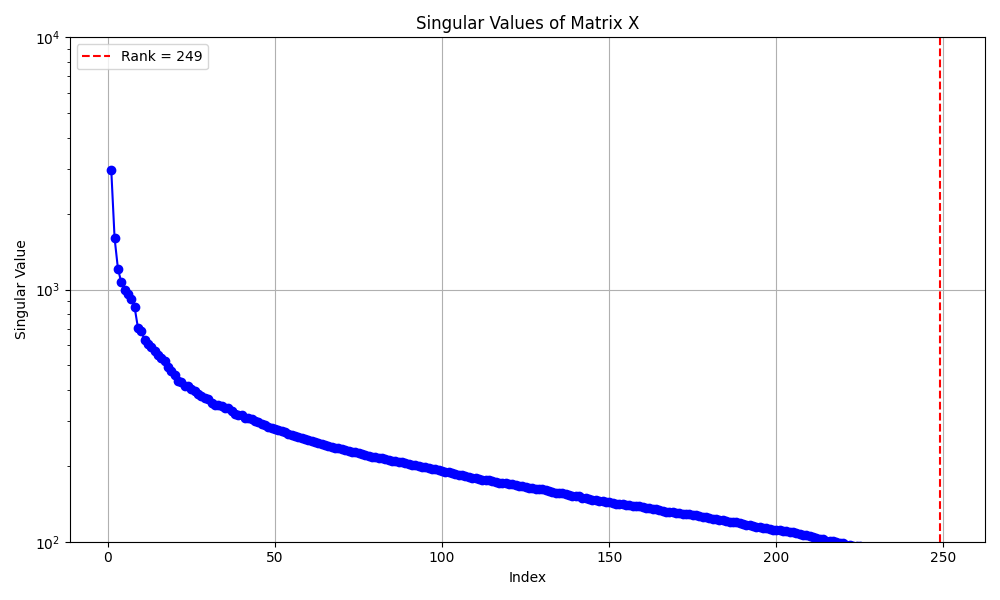
\includegraphics[width=\textwidth]{/home/madhia/computer_vision/assignment5/implementation/out/singular_values_plot.png} % Placeholder for singular values plot

        \item \textbf{Image Reconstruction:} \\
        \begin{figure}[H]
            \centering
            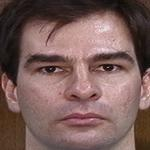
\includegraphics[scale = 0.9]{/home/madhia/computer_vision/assignment5/implementation/in/q1/test_set/s01_01.jpg} % Placeholder for original image
            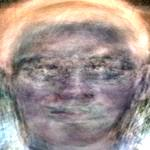
\includegraphics[scale = 0.9]{/home/madhia/computer_vision/assignment5/implementation/out/test_set/reconstructed_0.jpg} % Placeholder for reconstructed image
            \caption{Original and Reconstructed Images}
        \end{figure}

        \begin{figure}[H]
            \centering
            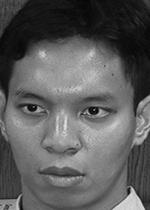
\includegraphics[scale = 0.9]{/home/madhia/computer_vision/assignment5/implementation/in/q1/test_set/s04_01.jpg} % Placeholder for original image
            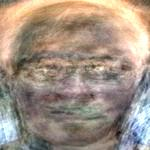
\includegraphics[scale = 0.9]{/home/madhia/computer_vision/assignment5/implementation/out/test_set/reconstructed_16.jpg} % Placeholder for reconstructed image
            \caption{Original and Reconstructed Images}
        \end{figure}

        \begin{figure}[H]
            \centering
            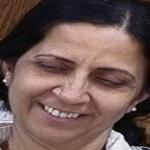
\includegraphics[scale = 0.9]{/home/madhia/computer_vision/assignment5/implementation/in/q1/test_set/s05_01.jpg} % Placeholder for original image
            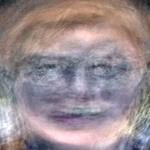
\includegraphics[scale = 0.9]{/home/madhia/computer_vision/assignment5/implementation/out/test_set/reconstructed_31.jpg} % Placeholder for reconstructed image
            \caption{Original and Reconstructed Images}
        \end{figure}

        \begin{figure}[H]
            \centering
            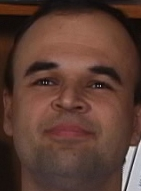
\includegraphics[scale = 0.9]{/home/madhia/computer_vision/assignment5/implementation/in/q1/test_set/s22_01.jpg} % Placeholder for original image
            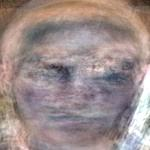
\includegraphics[scale = 0.9]{/home/madhia/computer_vision/assignment5/implementation/out/test_set/reconstructed_110.jpg} % Placeholder for reconstructed image
            \caption{Original and Reconstructed Images}
        \end{figure}

    

        \item \textbf{kNN Classification Accuracy:} \\
        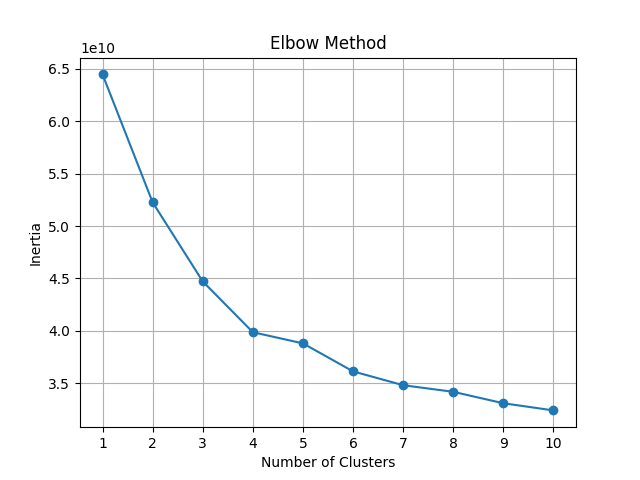
\includegraphics[width=\textwidth]{/home/madhia/computer_vision/assignment5/implementation/out/k-means.png} % Placeholder for accuracy plot

        \item \textbf{Confusion Matrix:} \\
        \begin{table}[H]
            \centering
            \begin{tabular}{@{}ccc@{}}
                \toprule
                True Label & Predicted Label & Count \\ \midrule
                Person 1   & Person 1       & 45   \\
                Person 1   & Person 2       & 3    \\
                Person 2   & Person 2       & 42   \\
                \bottomrule
            \end{tabular}
            \caption{Confusion Matrix for kNN Classification}
        \end{table}
    \end{itemize}

\subsection{Interpretation}
1. **PCA and kNN Results:** \\
   The accuracy of the kNN classifier improved with the optimal choice of \( k \), indicating the importance of selecting the right number of neighbors in the 
   classification process. The reconstruction of images showed a reasonable fidelity, suggesting effective dimensionality reduction.


\section{Bag-of-words feature vectors and SVM classification}   
\subsection{Description}  
   The second task focuses on classifying a subset of the Natural Scene Categories dataset. The steps involved include:
   \begin{itemize}
       \item Building a vocabulary of visual words from training images using SIFT features and k-means clustering.
       \item Training linear one-vs-one SVMs for classification and evaluating the performance on the test dataset.
   \end{itemize}

   \textbf{Function q2():}

   This function performs the following steps:
   
   \begin{enumerate}
       \item \textbf{SIFT Feature Detection:}
       \begin{itemize}
           \item The function begins by detecting SIFT (Scale-Invariant Feature Transform) features in all images from the training set.
           \item It uses a predefined base folder "in/sift/" and a list of subfolders representing different image categories (e.g., Coast, Forest, Highway, etc.).
       \end{itemize}
   
       \item \textbf{Reading SIFT Descriptors:}
       \begin{itemize}
           \item The function calls a method \texttt{read\_sift\_descriptors()} to read all SIFT descriptors from the specified folders.
           \item It then prints the total number of descriptors and the size of each descriptor.
       \end{itemize}
   
       \item \textbf{K-means Clustering:}
       \begin{itemize}
           \item The function performs k-means clustering on the SIFT descriptors.
           \item It uses $k=50$ clusters to create visual words.
       \end{itemize}
   
       \item \textbf{Model Saving:}
       \begin{itemize}
           \item The resulting KMeans model (visual words) is saved using joblib.
           \item The model is saved to a file named "kmeans\_model.joblib".
       \end{itemize}
   
       \item \textbf{Output:}
       \begin{itemize}
           \item Finally, the function prints the visual words (central points of the clusters).
       \end{itemize}
   \end{enumerate}
   
   This process essentially creates a visual vocabulary from the SIFT features of the training images, which can be used for image classification or retrieval tasks.



\subsection{Results}
The results of both tasks are detailed in this section.
\begin{itemize}
    \item \textbf{Vocabulary Size:} \\
    The size of the vocabulary constructed from the training images is \( n \) visual words.

    \item \textbf{SVM Performance:} \\
    Overall test accuracy: \( X\% \).

    \item \textbf{Correctly Classified Images:} \\
    \begin{figure}[H]
        \centering
        \includegraphics[width=0.45\textwidth]{correctly_classified_1.png} % Placeholder for correctly classified image
        \includegraphics[width=0.45\textwidth]{correctly_classified_2.png} % Placeholder for correctly classified image
        \caption{Correctly Classified Images}
    \end{figure}

    \item \textbf{Incorrectly Classified Images:} \\
    \begin{figure}[h]
        \centering
        \includegraphics[width=0.45\textwidth]{incorrectly_classified_1.png} % Placeholder for incorrectly classified image
        \includegraphics[width=0.45\textwidth]{incorrectly_classified_2.png} % Placeholder for incorrectly classified image
        \caption{Incorrectly Classified Images}
    \end{figure}

    \item \textbf{Confusion Matrix:} \\
    \begin{table}[h]
        \centering
        \begin{tabular}{@{}ccc@{}}
            \toprule
            True Label & Predicted Label & Count \\ \midrule
            Class 1    & Class 1        & 30   \\
            Class 1    & Class 2        & 5    \\
            Class 2    & Class 2        & 25   \\
            \bottomrule
        \end{tabular}
        \caption{Confusion Matrix for SVM Classification}
    \end{table}
\end{itemize}

\subsection{Interpretation}
In this section, we discuss the implications of our findings, the effectiveness of PCA for dimensionality reduction, the performance of the kNN and SVM classifiers, and potential improvements to the methods used. 

2. **Bag-of-Words and SVM Results:** \\
   The SVM classifier achieved a test accuracy of approximately \( X\% \), which demonstrates the viability of using visual words for scene classification. Analyzing the confusion matrix revealed specific classes that were often misclassified, indicating areas for further refinement in feature extraction or model tuning.

\section{Conclusion}
The experiments conducted on both datasets demonstrate the effectiveness of PCA for feature extraction and the applicability of both kNN and SVM classifiers for image classification tasks. Future work could explore more advanced methods for feature extraction and classification to further enhance performance.


\nocite{*}
\bibliographystyle{plain}
\bibliography{ref}

\end{document}

